%% The first command in your LaTeX source must be the \documentclass command.
\documentclass[acmtog]{acmart}
\usepackage[english,ngerman]{babel}
\usepackage[utf8]{inputenc} 

%% \BibTeX command to typeset BibTeX logo in the docs
\AtBeginDocument{%
  \providecommand\BibTeX{{%
    \normalfont B\kern-0.5em{\scshape i\kern-0.25em b}\kern-0.8em\TeX}}}
    
\copyrightyear{2024}
\acmYear{2024}
\citestyle{acmauthoryear}

\usepackage[figurename=Fig.]{caption}
\usepackage{csquotes}
\setcopyright{none}
\makeatletter
\renewcommand{\fnum@figure}{Abb. \thefigure}
\makeatother
\addto\captionsngerman{\renewcommand{\figurename}{Abb.}}
\settopmatter{printacmref=false} % Removes citation information below abstract
\renewcommand\footnotetextcopyrightpermission[1]{} % removes footnote with conference information in first column

\usepackage{minted}

%%
%% end of the preamble, start of the body of the document source.
\begin{document}

%%
%% The "title" command has an optional parameter,
%% allowing the author to define a "short title" to be used in page headers.
\title{Enterprise Architektur-Muster}

%%
%% The "author" command and its associated commands are used to define
%% the authors and their affiliations.
%% Of note is the shared affiliation of the first two authors, and the
%% "authornote" and "authornotemark" commands
%% used to denote shared contribution to the research.
\author{Julian Bruder}
\authornote{Alle Studierenden trugen zu gleichen Teilen zu dieser Arbeit bei.}
\author{Abdellah Filali}
\authornotemark[1]
\author{Luca Franke}
\authornotemark[1]
\affiliation{%
  \institution{Hochschule für Technik, Wirtschaft und Kultur Leipzig (HTWK Leipzig)}
  \streetaddress{Karl-Liebknecht-Str. 132}
  \city{Leipzig}
  \country{Deutschland}
  \postcode{04277}
}
%%
%% By default, the full list of authors will be used in the page
%% headers. Often, this list is too long, and will overlap
%% other information printed in the page headers. This command allows
%% the author to define a more concise list
%% of authors' names for this purpose.
\renewcommand{\shortauthors}{Bruder, Filali, Franke}

%%
%% The abstract is a short summary of the work to be presented in the
%% article.
\begin{abstract}
In diesem Papier werden verschiedene Enterprise Architektur-Muster und deren Rolle in modernen Geschäftsprozessen untersucht
und anschließend unter Einbeziehung technischer und struktureller Eigenschaften anhand ihrer Agilität bewertet.
Dabei orientiert sich die Reihenfolge der Betrachtung jener Architektur-Muster am historischen Verlauf derer Entwicklung und der Notwendigkeit dieser.
Genauer werden die monolithische Architektur, modulare monolithische Architektur, service-orientierte Architektur, Microservice-Architektur, Layered-Architecture,
Event-Driven Architecture, cloud-native Architektur und die Microkernel-Architektur betrachtet.

Insgesamt zeigt sich, dass klassische Enterprise Architektur-Muster zwar mit geringer initialer Komplexität punkten,
mit weiterführender Entwicklung allerdings Flexibilitätsprobleme bedingen.
Dem entgegen zeichnen sich die modernen Architektur-Muster durch hohe Agilität und damit hoher Flexibilität gegenüber den in der modernen Geschäftswelt ständig
wechselnden Anforderungen aus.
Besonders die cloud-native Architektur wird diesen Anforderungen gerecht.
\end{abstract}

\maketitle

\section{Einleitung}
% (Beschreibung von Kontext, Problemen, Anforderungen und Zielen)
Moderne Software-Systeme bestehen aus verschiedenen Komponenten \cite{evolutionOfDistributedSystems}.
Dabei nimmt der Nutzer des Systems jenes zwar als eine Software wahr, jedoch verbirgt sich in Realität meist eine Struktur aus
Software-Komponenten und deren Beziehungen hinter dieser Wahrnehmung - ein verteiltes Softwaresystem.
Die Art und Weise dieser Struktur und Beziehungen wird als Architektur bezeichnet.
Wie wird eine solche Architektur mit all ihren Anforderungen der modernen und schnelllebigen Geschäftswelt konstruiert?

Betrachten wir folgend ein Anwendungsbeispiel zur Motivation.
In einem Tech-Startup soll ein Backend für ein internationales E-Commerce-System entwickelt werden.
Dabei werden folgende Anforderungen gestellt:
\begin{itemize}
  \item Zukünftig viele Nutzer und hoher Traffic erwartet
  \item Geringes Kapital für Infrastruktur
  \item Rechtliche Regularien sind teilweise unklar
  \item Hohe Sicherheitsanforderungen aufgrund des Cash-Flows
  \item Agiles Team von acht fähigen Entwicklern
  \item Geldgeber wollen erste Auslieferung in zwei Wochen
\end{itemize}

Das Team arbeitet agil nach Scrum und einigt sich in einer der ersten Planungsphasen auf ein \textit{Minimum Viable Product} (kurz MVP) mit Bestellung, Bezahlung und Versand.
Abbildung \ref{fig:ecommerce-bpm} zeigt die Modellierung des Geschäftsprozesses für diesen MVP\@.
\begin{figure}[!h]
  \centering
  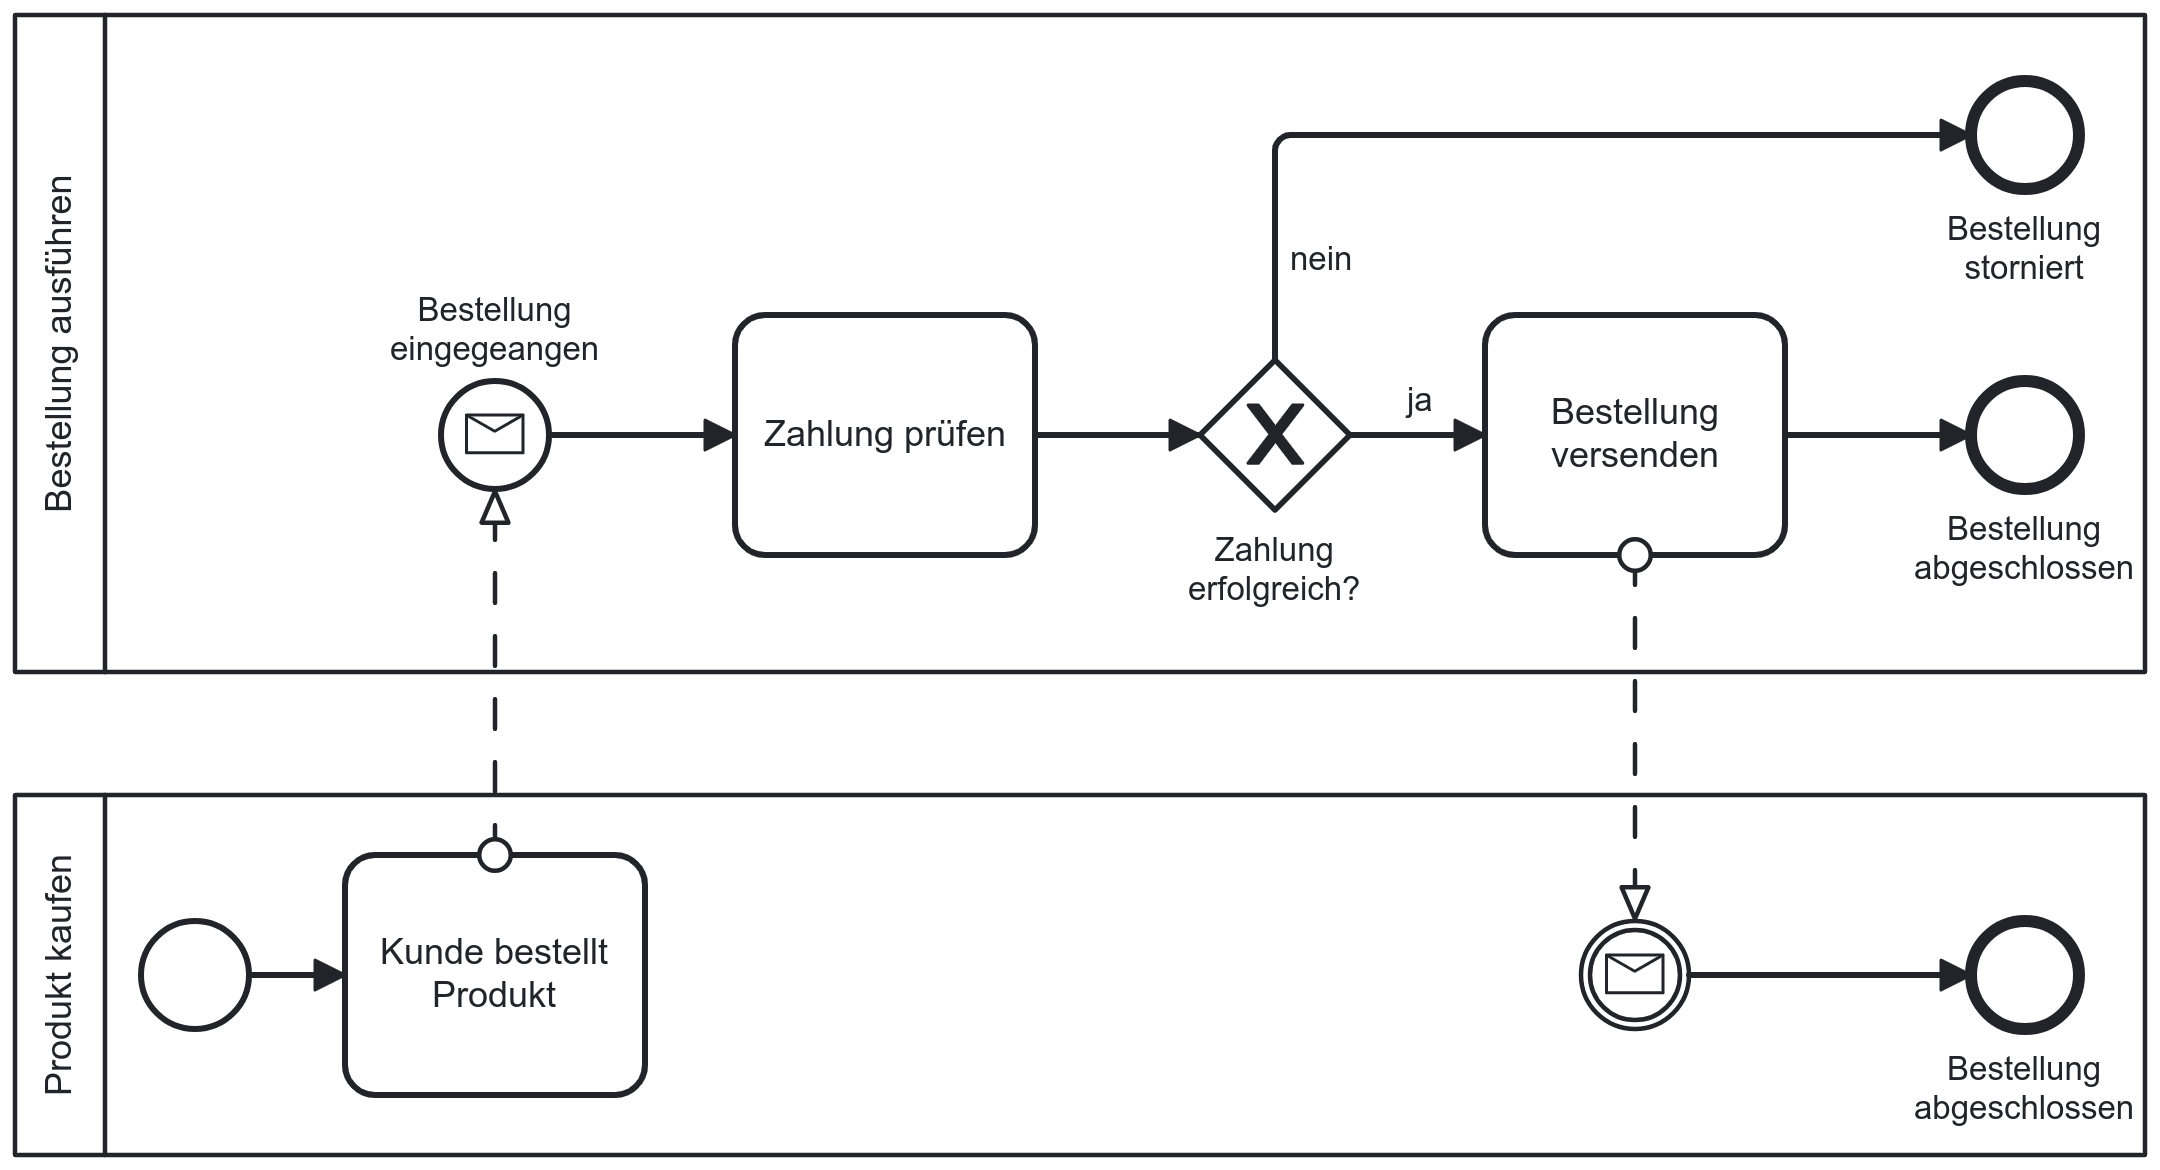
\includegraphics[width=\linewidth]{images/einleitung/ecommerce-order}
  \caption{Geschäftsprozessmodell des MVPs des E-Commerce-Beispiels}
  \label{fig:ecommerce-bpm}
\end{figure}
Die Anforderungen sind somit zwar grob strukturiert aber trotzdem ungewiss.
Die rechtlichen Regularien sind unklar, was zu späten technischen Änderungen führen kann.
Anfangs ist der erwartete Traffic vermutlich niedrig, später sollte dieser aus geschäftlicher Sicht bestenfalls ansteigen.
Wie wird der erwartet hohe Traffic aus infrastruktureller Sicht vorgesehen und finanziert?
Sind acht Entwickler ausreichend?
Kann nach zwei Wochen schon geliefert werden?

All diese Fragen betreffen nicht nur die Software, sondern offensichtlich auch das Geschäft.
Die Antworten dafür liefern Enterprise-Architekturen.
Deren Ziel ist die Ausrichtung von Geschäft und IT, also die Unterstützung des Geschäfts durch die IT und umgekehrt \cite{eaprinciples}.
Ein Enterprise Architektur-Muster ist dabei eine spezifische Strategie zur Umsetzung dieser Ausrichtung.
Erwähnenswert ist hier die Nähe zur Bedeutung des lateinischen Wortes \textit{architectura}.
Wörtlich übersetzt ist es die \textit{Wissenschaft der Baukunst} - meint aber sowohl das Produkt des Bauens als auch den Prozess des Bauens \footnote{https://www.duden.de/rechtschreibung/Architektur, abgerufen am 17.01.2025}.
In Bezug dazu kann die Enterprise-Architektur also als Vision einer grundlegenden Struktur und Beziehungen von Komponenten eines Systems betrachtet werden.
Wichtig ist hierbei die Abgrenzung zur Software-Architektur, der grundlegenden Struktur und Beziehungen von Teilen einer Software.

Im Verlauf der Arbeit werden verschiedene Enterprise Architektur-Muster und deren Rolle in modernen Geschäftsprozessen untersucht
und anschließend unter Einbeziehung technischer und struktureller Eigenschaften anhand ihrer Agilität bewertet.
Dabei wird auch immer auf das eingangs erwähnte und in Abbildung \ref{fig:ecommerce-bpm} dargestellte E-Commerce-Beispiel zurückgegriffen.
Die Arbeit ist wie folgt strukturiert:

Zunächst wird in Abschnitt TODO auf die monolithische Architektur eingegangen, bevor die Modularisierung des Monolithen in Abschnitt TODO diskutiert wird.
Danach wird in Abschnitt TODO die service-orientierte Architektur betrachtet.
Folgend wird in Abschnitt TODO die Microservice-Architektur diskutiert.
Anschließend wird in Abschnitt TODO untersucht, wie eine Schichten-Architektur andere, dienst-basierte Architekturen ergänzen kann.
Daraufhin werden sowohl die event-basierte Architektur in Abschnitt TODO als auch die cloud-native Architektur in Abschnitt TODO erläutert.
Als letztes Architektur-Muster wird in Abschnitt TODO die Microkernel-Architektur betrachtet.
Abschließend werden die Architekturen in Abschnitt TODO nach technischen und agilen Kriterien verglichen und folglich die Ergebnisse dieser Arbeit zusammengefasst.

\section{Klassische Enterprise-Architekturen}
\subsection{Monolithic Architecture}
Der Begriff \textit{Monolith}, abgeleitet aus dem Altgriechischen und mit der Bedeutung
\textit{einheitlicher Stein}, wird in der Softwarearchitektur verwendet, um ein Designmuster
zu beschreiben, bei dem die gesamte Funktionalität einer Anwendung in einem einzigen,
zusammenhängenden System integriert ist.
In dieser Architektur übernimmt ein einzelner Prozess die Ausführung der gesamten Anwendung \cite[1]{mono}.

Anwendungen, die diesem Architekturansatz folgen, bestehen aus eng miteinander verknüpften
Komponenten, die wechselseitig voneinander abhängen.
Diese Komponenten können weder unabhängig betrieben noch, in bestimmten Fällen,
isoliert kompiliert werden \cite[485]{mono3}.

\begin{figure}[h!]
  \centering
  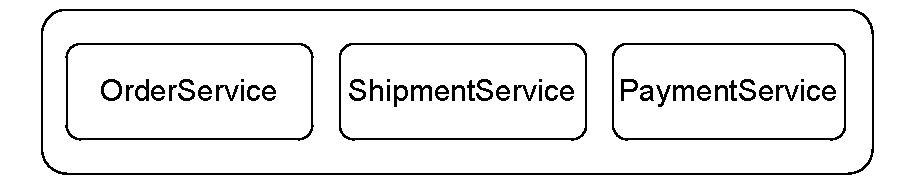
\includegraphics[width=0.4\textwidth]{images/mono/mono.pdf}
  \caption{Monolith Architektur}
  \label{fig:mono}
\end{figure}

Diese Architektur bietet insbesondere für kleinere Anwendungen mehrere Vorteile,
wie etwa eine vereinfachte Testbarkeit, Logging, Deployment und Debugging. Ein
weiterer Vorteil besteht darin, dass keine separate Datenbanksynchronisation
erforderlich ist, da sämtliche Daten in einer einzigen Datenbank gespeichert
werden \cite[2]{mono4}.

Betrachten wir das E-Commerce-Beispiel.
Dafür definieren wir drei Klassen:
\begin{itemize}
  \item \texttt{OrderService}: Klasse, die die Bestellungen verwaltet
  \item \texttt{PaymentService}: Klasse, die die Zahlungen abwickelt
  \item \texttt{ShipmentService}: Klasse, die die Lieferungen initiiert
\end{itemize}

Die Kommunikation zwischen den Klassen erfolgt über Methodenaufrufe. In diesem
Zusammenhang stellt die Klasse \texttt{OrderService} die zentrale Komponente dar,
die die Methoden anderer Klassen nutzt, um den Bestellprozess zu steuern. Ein
wesentlicher Vorteil dieses Ansatzes liegt in der einfachen Kommunikation
zwischen den Komponenten.
Durch den direkten Einsatz von Methodenaufrufen
wird die Komplexität verringert, die typischerweise mit der Interaktion zwischen
verschiedenen verteilte Systemen verbunden ist.

Eine beispielhafte Implementierung des Payment-Service in einer monolithischen
Architektur ist im Anhang dargestellt.
Der vollständige Quellcode kann zudem bei GitHub
\footnote{https://github.com/Beleg-6-EAP/demo-monolith-ecommerce} eingesehen werden.

Mit dem Wachstum und der zunehmenden Komplexität der Code-Basis treten jedoch
einige Nachteile auf.
Änderungen an einer Komponente können unerwartete kaskadierende
Fehler auslösen, was die Weiterentwicklung in kleinen, autonomen Teams erschwert
und verlangsamt.

Ein weiterer Nachteil ergibt sich aus der engen Kopplung zwischen den Komponenten,
die durch direkte Methodenaufrufe entsteht.
Änderungen an der Implementierung oder
der Signatur einer Methode können in der Folge die gesamte Anwendung beeinflussen.

Zudem wird die Wiederverwendung von Funktionalitäten erschwert, da die Komponenten
stark miteinander verknüpft sind.
Dies führt zu einer Duplizierung von Code, was die Kosten für Änderungen erhöht,
da diese an mehreren Stellen vorgenommen werden müssen.

Die daraus resultierende Komplexität und die erschwerte Wartung führen zu längeren
Iterationen.
Da das Deployment nur als Ganzes erfolgen kann, und die Iterationen
sich verlängern, kommt es zu seltenen Auslieferungen neuer Features.

Ein weiteres Problem liegt in der erschwerten horizontalen Skalierung, da die Anwendung
nur als Ganzes skaliert werden kann.
Dies stellt eine Herausforderung dar, da bei wachsenden
Anforderungen die gesamte Anwendung skaliert werden muss, anstatt einzelne Komponenten unabhängig
voneinander zu skalieren.

Insgesamt ist die monolithische Architektur eine geeignete Lösung für
kleinere Anwendungen, jedoch weniger geeignet für größere Systeme, da sie die Agilität und
Flexibilität erheblich einschränken kann.

\subsection{Modular Monolith}
Das Hauptproblem der zuvor beschriebenen Architektur liegt in der engen Kopplung der Komponenten,
was zu einer erhöhten Komplexität und begrenzten Flexibilität führt.
Die Modular Monolithic Architecture stellt eine Weiterentwicklung der Monolithic Architecture dar,
indem sie die Vorteile des monolithischen Ansatzes bewahrt und gleichzeitig die Nachteile
der engen Kopplung verringert.

In diesem Architekturmodell wird die Code-Basis in mehrere Module unterteilt, die jeweils
eine spezifische Teilfunktionalität der Anwendung implementieren.\cite[11]{modular-mono2}.

Die Modularisierung trägt zudem zur Reduzierung der Komplexität bei und ermöglicht eine bessere
Organisation der Code-Basis, was sich positiv auf die Wartbarkeit der Anwendung auswirkt \cite[23 - 24]{modular-mono4}.

\begin{figure}[h!]
  \centering
  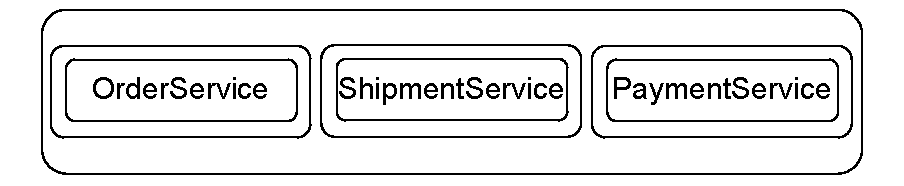
\includegraphics[width=0.4\textwidth]{images/mono/mono-example.pdf}
  \caption{Modular Monolith Architektur}
  \label{fig:modular-mono}
\end{figure}

Betrachten wir erneut das E-Commerce-Beispiel.
Diesmal wird die Anwendung in drei Hauptmodule aufgeteilt (Siehe Abb. ~\ref{fig:modular-mono}):
\begin{itemize}
  \item \texttt{order}: Modul, das für die Verwaltung der Bestellungen verantwortlich ist
  \item \texttt{payment}: Modul, das für die Abwicklung der Zahlungen verantwortlich ist
  \item \texttt{shipment}: Modul, das für die Initiierung der Lieferungen verantwortlich ist
\end{itemize}

Wie die Abbildung \ref{fig:modular-mono} zeigt, jedes Service ist in einem eigenen Modul gekapselt.
Eine beispielhafte Implementierung der Payment-Service innerhalb des Moduls \texttt{payment}
ist im Anhang zu finden.
Die vollständige Implementierung des E-Commerce-Beispiels ist bei GitHub
\footnote{https://github.com/Beleg-6-EAP/demo-modulith-ecommerce} zu finden.

Durch die Modularisierung sind die Komponenten weniger eng miteinander gekoppelt, was eine
verbesserte Zusammenarbeit in kleinen, autonomen Teams fördert, im Vergleich zu traditionellen
monolithischen Ansätzen.

Ein Nachteil bleibt jedoch bestehen: Die Anwendung muss weiterhin als Ganzes deployed werden,
was die Iterationen verlangsamt.
Zudem bleibt die horizontale Skalierung weiterhin erschwert,
und die Funktionalitäten können nicht wiederverwendet werden, da sie immer noch Teil einer
einzigen Anwendung sind und eng miteinander gekoppelt bleiben.
\section{Moderne Enterprise-Architekturen}

\subsection{Microkernel Architecture}\label{subsec:microkernel-architecture}
Die Microkernel Architecture ist ein Architekturmuster, was sich durch Erweiterbarkeit, Flexibilität und vor allem Isolation der Funktionalitäten auszeichnet.
Wie in Abbildung~\ref{fig:microkernel} dargestellt, enthält ein Microkernel zwei wesentliche Komponenten: Den Kern der Anwendung,der die wichtigsten grundlegenden Funktionalitäten bereitstellt und Module oder auch Plugins,
die diesen Kern um Features erweitern~\cite[21-22]{architecturePatterns}.


\begin{figure}[!h]
  \centering
  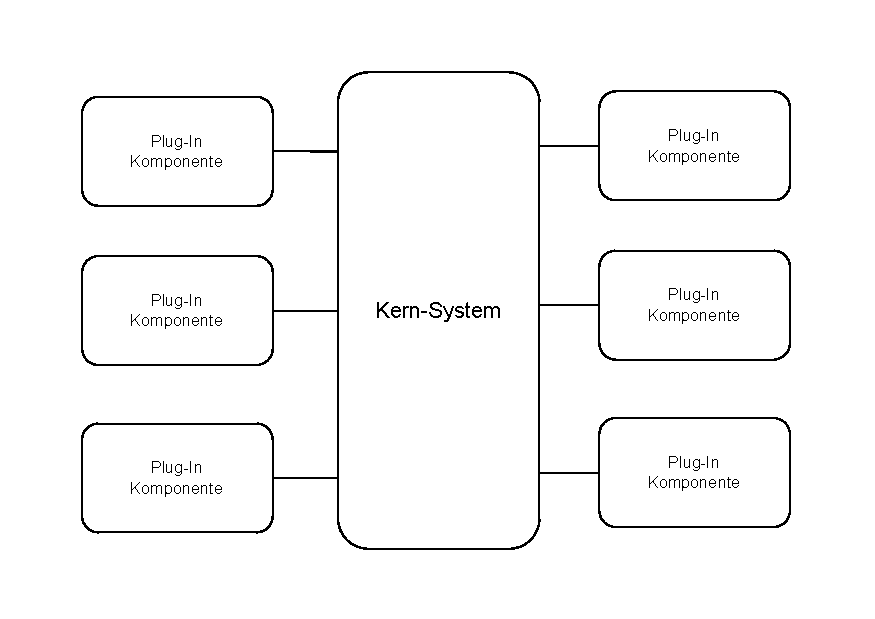
\includegraphics[width=\linewidth]{images/microkernel/microkernel}
  \caption{Aufbau einer Microkernel Architecture}
  \label{fig:microkernel}
\end{figure}

Der Kern der Anwendung implementiert dabei meist nur die minimalste Funktionalität, um die Anwendung oder das System lauffähig zu machen.
Alle weiteren Funktionalitäten werden in Modulen implementiert, die auf den Kern aufbauen.
Module sind meist unabhängig voneinander aufgebaut, es kann jedoch auch vorkommen, dass manche Module von anderen abhängig sind.
Best practice für die Entwicklung von Microkernel Architekturen ist es, die Kommunikation zwischen einzelnen Modulen so gering wie möglich zu halten, um Probleme durch Abhängigkeiten zu vermeiden.
Dadurch sind Module untereinander lose gekoppelt und können unabhängig voneinander entwickelt, getestet und deployed werden~\cite[22]{architecturePatterns}.

Die Plugins können über verschiedene Wege mit dem Kern verbunden werden.
Eine genaue Spezifikation zum Verbinden der Plugins mit dem Kern gibt es aber laut Architekturschema nicht, diese Entscheidung ist dem Entwickler überlassen und entsprechend der Anforderungen und Anwendungsumgebung zu treffen.
Unabhängig von der Art der Verbindung definiert der Kern die Schnittstellen, um Plugins anzubinden.
Diese Verbindung könnte dann beispielsweise über Web-Services, Messaging oder am einfachsten über direkte Objekt-Instanziierung innerhalb der gleichen Anwendung stattfinden~\cite[22-23]{architecturePatterns}.

Zwischen Plugins und Kern werden Verträge definiert, die die Kommunikation zwischen den beiden Komponenten regeln.
Diese Verträge können in Form von Interfaces, Klassen oder auch Datenstrukturen definiert werden.
Alle Plugins, müssen sich zwingend an die definierten Verträge halten, um mit dem Kern kommunizieren zu können.
Alternativ können auch Adapter verwendet werden, um bestehende Plugins an den Kern und die Verträge anzupassen, wodurch wiederrum die lose Kopplung der Komponenten verbessert wird.

Durch diesen Aufbau ergibt sich jedoch das Problem, dass der Kern jederzeit über Verfügbarkeit und Erreichbarkeit der Plugins informiert sein muss.
Um dieses Problem zu lösen, kann eine zentrale Plugin-Registry verwendet werden.
Diese Registry enthält alle aktuell verfügbaren Plugins sowie die dazugehörigen relevanten Informationen wie zum Beispiel Name des Service, Verträge, Verbindungsdetails, etc.
Der Kern der Anwendung kann dann zur Laufzeit auf diese Registry zugreifen und Plugins dynamisch laden~\cite[22]{architecturePatterns}.

Microkernel Architekturen können auch in andere Architekturmuster eingebettet werden, falls es nicht möglich sein sollte die gesamte Software in diesem Architekturmuster aufzubauen.
Vor allem Teile von Anwendungen, die stark erweiterbar sein müssen, eignen sich gut für die Verwendung der Microkernel Architektur.

Ein klarer Vorteil dieses Architekturmusters ist die schnelle Reaktionsfähigkeit auf äußere Änderungen, da Anpassungen aufgrund der losen Kopplung größtenteils nur in den isolierten Modulen vorgenommen werden.
Der Kern der Anwendung ist in den meisten Fällen schnell stabil und benötigt selten im Laufe der Entwicklung weitere Angleichungen.
Geänderte Module können je nach Implementierung auch zur Laufzeit geladen oder hinzugefügt werden, was mögliche Downtime von bereits ausgelieferter Software minimiert~\cite[25]{architecturePatterns}.

Ein Beispiel dafür stellt die Entwicklung von Betriebssystem-Kernels dar, die auch namensgebend für dieses Architekturmuster ist.
Deren Kern Komponenten sind in der Regel sehr stabil und implementieren vor allem grundlegende Funktionen wie Speicherverwaltung, Prozessverwaltung und I/O-Operationen.
Weitere low-level Funktionalitäten wie beispielsweise Geräte Treiber oder Dateisysteme werden als Module in den Kernel geladen und können bei Bedarf hinzugefügt oder entfernt werden, was vor allem für die Unterstützung neuer Hardware wichtig ist.

Auch Entwicklungsumgebungen in der Softwareentwicklung nutzen oft Microkernel Architekturen, um die Support für verschiedene Programmiersprachen und Frameworks zu ermöglichen.

Zwar bietet das Beispiel der E-Commerce Anwendung keinen klassischen Anwendungsfall für Microkernel Architekturen, jedoch kann die Verwendung von Microkernel Architekturen in Teilen der Anwendung trotzdem sinnvoll sein.
Sowohl Zahlungs- als auch Versandfunktionalitäten könnten, wie in Abbildung~\ref{fig:ecommerce-microkernel} dargestellt, in Module ausgelagert werden, um die Anwendung durch weitere Dienstleister erweitern zu können.

\begin{figure}[!h]
  \centering
  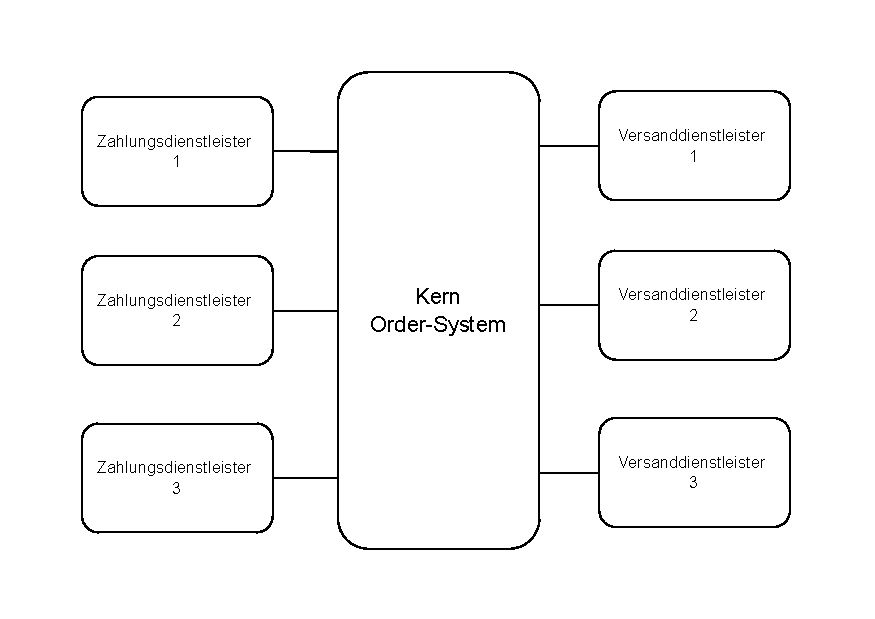
\includegraphics[width=\linewidth]{images/microkernel/ecommerce-mikrokernel}
  \caption{Aufbau der E-Commerce Anwendung mit Microkernel Architektur}
  \label{fig:ecommerce-microkernel}
\end{figure}

Logik zum Verarbeiten der Zahlungen und Versandinformationen wird dann in den Modulen implementiert, die auf den Kern der Anwendung aufbauen.
Dabei ist jedoch ein Großteil der Business-Logik im Kern der Anwendung enthalten, was nicht dem eigentlichen Gedanken der Microkernel Architektur entspricht.

Abgesehen davon erhöhen Microkernel Architekturen inhärent die Testbarkeit der Software, da Module nur lose Kopplung gekoppelt sind.
Jedes Modul kann unabhängig voneinander getestet werden und fehlende Module durch Stubs ersetzt werden, wodurch sich während der Entwicklung auf einzelne Module isoliert konzentriert werden kann~\cite[26]{architecturePatterns}.
Weiterhin können Verhaltensweisen von anderen Modulen durch Mocks simuliert werden, um Testzustände zu erzeugen und das Verhalten der Anwendung zu verifizieren.
In Agilen Umgebungen, in denen das Testen von Software eine wichtige Rolle spielt, ist die Verwendung von Microkernel Architekturen daher besonders sinnvoll.

Eine Herausforderung bei der Verwendung von Microkernel Architekturen kann jedoch der Entwurf der Kern-Komponente darstellen.
Da alle anderen Module auf den Kern aufbauen, muss dieser sehr sorgfältig und stabil entwickelt werden, um die Funktionalität der gesamten Anwendung zu gewährleisten.
Diese Rolle sollten vor allem erfahrene Entwickler übernehmen, da sich Design-Fehler der Kern-Komponente oder Verträge negativ auf die Entwicklung der Module auswirken können.
Sollte der Kern der Anwendung angepasst werden, so müssen tendenziell auch alle Module überprüft oder aktualisiert werden, was zu erheblich erhöhten Entwicklungszeiten führen kann und zuvor gewonnene Vorteile der Microkernel Architektur zunichte macht.

Aufgrund der initial hohen Komplexität, die mit der Entwicklung des Kerns einhergeht, stellt die Mikrokernel Architektur nicht die beste Wahl dar, wenn es darum geht schnell eine erste Version der Software auf den Markt zu bekommen.
Die wesentlichen Vorteile, die die Microkernel Architektur bietet, zeigen sich erst im späteren Verlauf der Entwicklung, wenn die Anwendung erweitert werden muss.
Sowohl Iterationen als auch Auslieferungszeiten sind dann sehr kurz, da Module unabhängig voneinander entwickelt werden und die Anwendung schnell an neue Anforderungen angepasst werden kann.
Diese Vorteile können die Architektur in ausgewählten Anwendungsfällen sehr geeignet für agile Entwicklungsumgebungen machen.

\subsection{Microservice-Architecture}
\label{subsec:microservice}

\subsection{Event-Driven Architecture}
\label{subsec:eda}
Die Event-Driven Architecture wählt als Basis einen anderen Ausgangspunkt als die bisherigen Architekturmuster.
Während bei letzteren Komponenten Dienste bereitstellen, welche von anderen Komponenten explizit genutzt werden,
verhalten sich Dienst-bereitstellende Komponenten in der Event-Driven Architecture reaktiv,
werden also implizit von Dienst-konsumierenden Komponenten genutzt \cite{garlanShawImplizit}.
Ein System reagiert somit asynchron auf Zustandsänderungen, also Ereignisse in diesem System \cite{eda}.
Die in dieser Architektur minimalen Einheiten, welche Informationen einer Zustandsänderung kapseln, werden \textit{Events} genannt.
Die Idee der impliziten Behandlung von Ereignissen ist nicht neu und taucht erstmals 1994 im von Garlan und Shaw publizierten Papier
\textit{\enquote{An introduction to Software Architecture}} auf.

Betrachten wir im Folgenden die Basis-Bestandteile der Event-Driven Architecture:
\begin{itemize}
  \item Ereignis (englisch \textit{Event}): Kapselt Information einer Zustandsänderung eines Systems
  \item Produzent (englisch \textit{Producer}): Komponente, die Event erzeugt
  \item Herausgeber (englisch \textit{Publisher}): Komponente, die, von Produzenten erzeugte, Events publiziert
  \item Konsument (englisch \textit{Consumer}): Komponente, die auf publizierte Events reagiert
  \item Vermittler (englisch \textit{Mediator}): Komponente zwischen Produzenten und Konsumenten - filtert Events und verteilt diese auf Konsumenten
  \item Event-Bus: Oft auch \textit{Event-Broker} genannt - bietet die Infrastruktur für die Gesamtheit der Vermittler
\end{itemize}
Abstrakt kann ein Event als Vertrag zwischen Produzenten und Konsumenten am Event-Bus betrachtet werden.
Der Konsument nutzt die Spezifikation des Events am Bus, der Produzent implementiert jene Spezifikation.
Abbildung \ref{fig:eda} stellt diesen Vertrag dar.

\begin{figure}[!h]
  \centering
  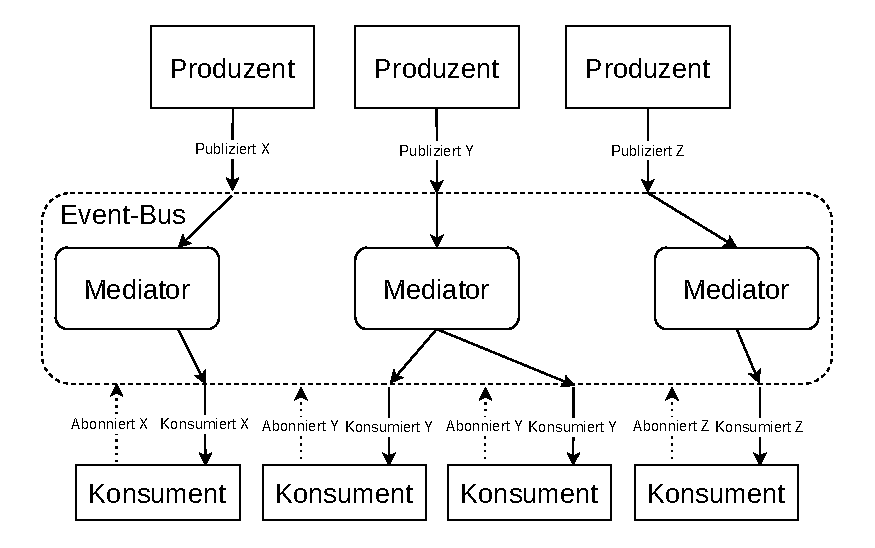
\includegraphics[width=\linewidth]{images/eda/eda.drawio}
  \caption{Vertrag zwischen Produzenten und Konsumenten am Event-Bus}
  \label{fig:eda}
\end{figure}

Durch den Vertrag weisen die Events am Event-Bus starke Kohäsion und somit lose Kopplung auf.
Diese lose Kopplung minimiert nicht nur kaskadierende Fehler, sondern ermöglicht kleinen und autonomen Entwickler-Teams
die klare Abgrenzung von Features und folglich einfach definierbare Iterationen - eine Menge von Events, deren Erzeugung und Konsumierung.

Weiter sind Events oft nah an dem, was Ereignisse in realen Prozessen sind, also domain-driven.
Gebündelt ermöglichen obige Punkte die kontinuierliche Auslieferung von Software in kurzen Intervallen.

Außerdem garantiert die asynchrone Behandlung von Ereignissen zusammen mit der loosen Kopplung hohe Skalierung und die Möglichkeit für Echtzeit-Software.
Daher sind Event-Driven Architekturen besonders für datenintensive Echtzeit-Anwendungen wie IoT (Internet of Things) und Analytics geeignet \cite{iotEda}.

Betrachten wir erneut das E-Commerce-Beispiel aus der Einleitung.
Dafür definieren wir drei Arten von Events:
\begin{itemize}
  \item \texttt{OrderCreated}: Ein Event, das genau dann erzeugt wird, wenn eine neue Bestellung aufgegeben wird
  \item \texttt{PaymentProcessed}: Ein Event, das genau dann erzeugt wird, wenn der Bezahlvorgang abgeschlossen wird
  \item \texttt{ShipmentInitiated}: Ein Event, das genau dann erzeugt wird, wenn die Bestellung versandt wird
\end{itemize}

Analog zur Microservice-Architektur teilen wir die Funktionalitäten in drei verschiedene Dienste auf: \texttt{OrderService}, \texttt{PaymentService} und \texttt{ShipmentService}.

\begin{figure}[!h]
  \centering
  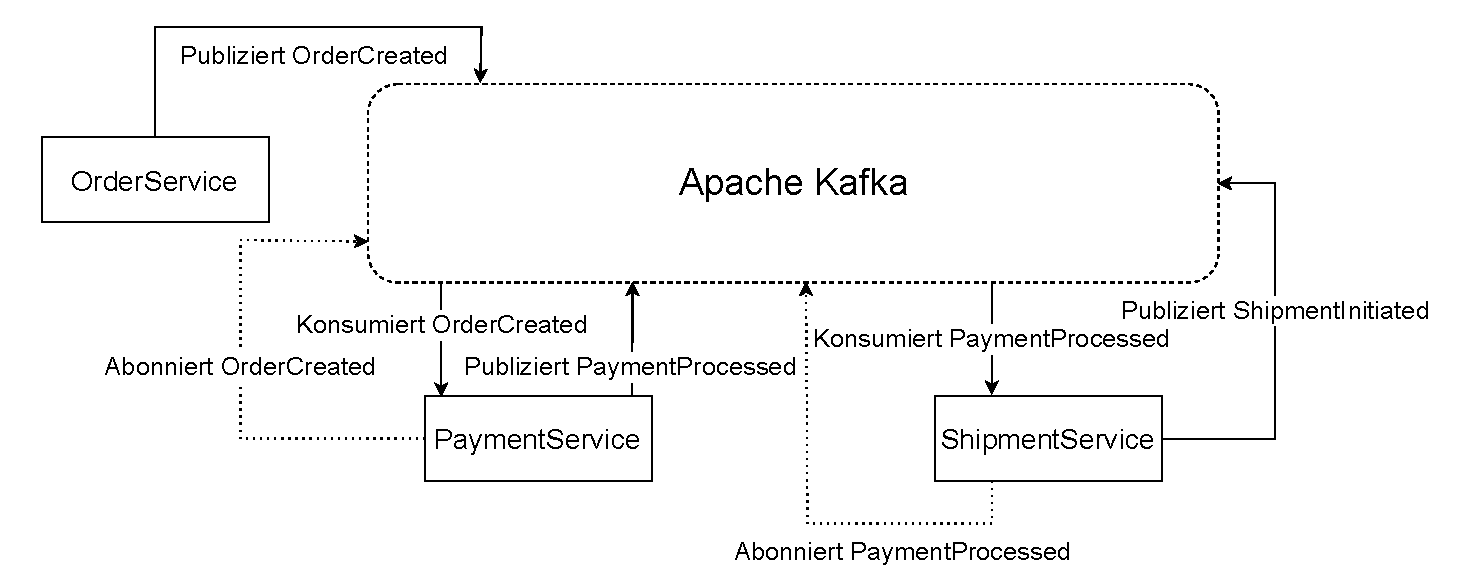
\includegraphics[width=\linewidth]{images/eda/eda-ecommerce.drawio}
  \caption{E-Commerce-Beispiel mit Event-Driven Architecture}
  \label{fig:edaecommerce}
\end{figure}
Wie Abbildung \ref{fig:edaecommerce} zeigt, sind alle drei Dienste Produzenten und Publisher, erzeugen also Events und veröffentlichen diese.
Die Dienste \texttt{PaymentService} und \texttt{ShipmentService} sind zudem Konsumenten,
sodass ersterer auf Events des Typs \texttt{OrderCreated} und zweiterer auf Events des Typs \texttt{ShipmentInitiated} reagiert.
Eine beispielhafte Implementierung des \texttt{PaymentService} mit Apache Kafka als Event-Broker ist im Anhang \ref{app:code:eda:paymentservice} zu finden.
Die vollständige Implementierung des E-Commerce-Beispiels ist bei GitHub \footnote{https://github.com/Beleg-6-EAP/demo-eda-ecommerce} zu finden.

Das Beispiel zeigt, dass die Event-Driven Architektur mit weiteren agilen Strukturen wie Microservices kombiniert werden kann, was die Agilität der Architektur weiter erhöht.
Die damit einhergehende Komplexität stellt teilweise hohe Anforderungen an die Entwickler.
Aufgrund der Asynchronität der Behandlung von Ereignissen ist die Testung des Systems meist schwer und die Fehlerbehandlung essentiell.
Mögliche Problemquellen schließen dabei unter anderem Event-Verlust, erhöhte Latenz und Inkonsistenz ein.
Die hohen Anforderungen an die Entwickler verlangen viel Vertrauen in jene, einer der zentralen Punkte des agilen Manifests \cite{agileManifesto}.
Insgesamt weist die Event-Driven Architecture also eine sehr hohe Agilität auf und ist damit besonders für moderne Software und ihre stetig wechselnden Anforderungen geeignet.

\subsection{Cloud-Native Architecture}
Die Cloud-Native Architecture beruht auf der Annahme, dass die Infrastruktur in ständigem Wandel ist und die Auslagerung jener in die Cloud mehr Agilität schafft \cite{cloudNative}.
Als Cloud wird in diesem Fall die Infrastruktur eines oder mehrerer Cloud-Vendors bezeichnet.
Ein Cloud-Vendor bietet seine Infrastruktur und deren Verwaltung dabei gegen eine Gebühr an.
Unter anderem offeriert er:
\begin{itemize}
  \item Die globale Nutzung von Ressourcen durch Geo-Redundanz und somit starke Verteilung sowie hohe Verfügbarkeit von Software,
  \item dynamische Skalierung bereitgestellter Ressourcen basierend auf der Nachfrage von Software (Auto-Scaling),
  \item nutzungsbedingte Gebühren, sodass nur tatsächlich verwendete Ressourcen bezahlt werden (Pay-as-you-go),
  \item unterbrechungsfreie Updates von Software (Zero Downtime).
\end{itemize}

Als cloud-nativ wird hierbei all jene Software bezeichnet, welche explizit für die Cloud entwickelt wurde.
Grundsätzlich baut die cloud-native Architektur auf die in diesem Artikel bereits in Abschnitt \ref{subsec:microservice} erklärte Microservice-Architektur und die
in Abschnitt \ref{subsec:eda} erklärte Event-Driven Architecture auf.
Zusätzlich kommen sogenannte \textit{Fully Managed Cloud-Services} hinzu, was cloud-spezifische und vom Cloud-Vendor vollständig verwaltete Dienste sind.
Jene umfassen alle von Datenbanken über Message-Queues bis hin zu Serverless-Functions und viele mehr.
Charakterisiert werden diese durch die Eigenschaft, dass sich der Entwickler gänzlich auf die Business-Logik konzentrieren kann, da der Cloud-Provider
die vollständige Verwaltung der Infrastruktur übernimmt.
Zentral dabei ist der Aspekt der Containerisierung, bei welchem jede Komponente eines Systems in einen Container gepackt wird.
Der Cloud-Vendor kann die Gesamtheit der Container dann dynamisch orchestrieren und somit gezielt den Ressourcenverbrauch optimieren.

Im Folgenden greifen wir erneut das Beispiel E-Commerce aus der Einleitung auf und betrachten die Anpassung der in
Abschnitt \ref{subsec:eda} angewendeten Event-Driven-Architecture auf die Cloud-Native Architecture mit Cloud-Vendor AWS\@.

Dabei ersetzen wir den dort verwendeten Broker durch eine \textit{Event-Bridge} \footnote{https://aws.amazon.com/de/eventbridge/, abgerufen am 06.01.2025}
- ein serverless Cloud-Service von AWS zum Routen von Ereignissen.
Weiter werden die drei Services für Aufgeben einer Bestellung, Bearbeitung der Bezahlung und Initiierung des Versands als \textit{Lambda} \footnote{https://aws.amazon.com/de/lambda/, abgerufen am 06.01.2025},
also Serverless-Function implementiert.
Abbildung \ref{fig:cloudnativeecommerce} stellt diese cloud-native Architektur dar.
Eine beispielhafte Implementierung des \texttt{ProcessPaymentLambda}s ist im Anhang \ref{app:code:cloudnative:paymentservice} und auf GitHub\footnote{https://github.com/Beleg-6-EAP/demo-cloud-native-ecommerce} zu finden.
\begin{figure}[!h]
  \centering
  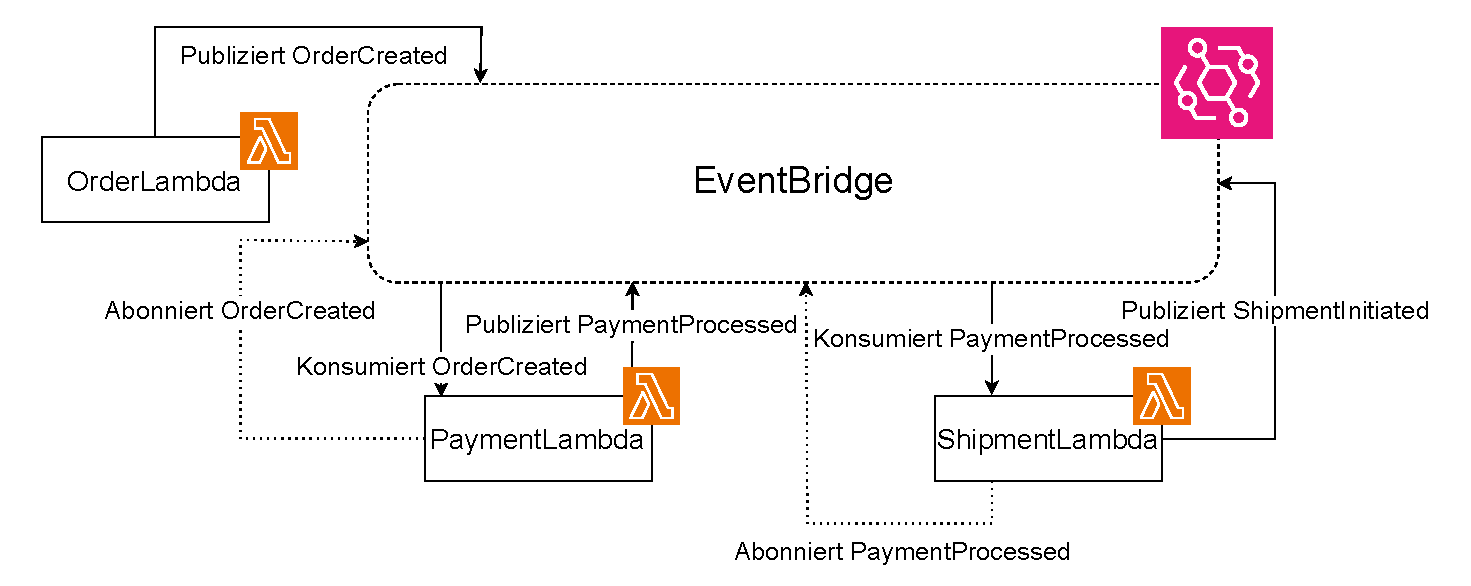
\includegraphics[width=\linewidth]{images/cloud-native/cloud-native-ecommerce.drawio}
  \caption{E-Commerce-Beispiel mit Cloud-Native Architecture}
  \label{fig:cloudnativeecommerce}
\end{figure}

Damit kombiniert die Cloud-Native Architecture die agilen Vorteile der Microservice- und Event-Driven Architecture.
Weiter ermöglichen die Cloud-Vendors nahtlose und einfache Möglichkeiten zur Auslieferung der Software,
wie beispielsweise Code-Deploy \footnote{https://aws.amazon.com/de/codedeploy/, abgerufen am 06.01.2024} bei AWS\@.
Die Option, allen Fokus von der Infrastruktur auf die Entwicklung zu legen, ermöglicht gemeinsam mit der einfachen Auslieferung kurze Iterationen in agilen Teams
und somit noch kürzere Zyklen in der Bereitstellung von Software.
Dabei ist besonders die Time-to-Market sehr gering, sodass Tech-Start-Ups häufig cloud-native Architekturen für ihre Software wählen. % TODO: Quelle!

Nicht zu vergessen ist zudem die extrem hohe Flexibilität der eingesetzten Ressourcen durch das Auto-Scaling.
Das damit verbundene Pay-as-you-go ermöglicht weiter auch finanzielle Agilität, wodurch zum Beispiel keine Vorab-Investitionen für Infrastruktur notwendig sind.
Jedoch ist zu betonen, dass aufgrund dessen auch Kostenrisiken durch möglicherweise unerwartete, extrem hohe Nachfrage der Software bestehen.
Ebenfalls nicht zu vernachlässigen ist die enge Bindung an den Cloud-Vendor durch Verwendung seiner spezifischen Cloud-Dienste.
Im Fall einer Migration zu einem anderen Cloud-Vendor könnten sowohl hohe Kosten beim vorherigen Cloud-Vendor, als auch Entwicklungskosten durch die notwendige
Anpassung der genutzten spezifischen Cloud-Dienste anfallen.
Obwohl das die Wahl des Cloud-Anbieters und der damit verbunden Entwicklung weniger agil macht, gilt die Cloud-Native Architecture besonders aufgrund der Auslagerung
der Infrastruktur als eine - und vermutlich die agilste Architektur für moderne Software.

\section{Fallstudien und Praxisbeispiele}
Blah \ldots

\section{Diskussion}

\section{Zusammenfassung und Ausblick}
%(Überblick über die gesamte Arbeit, Rückführung auf Aussagen aus Kapitel 1 durchführen, offene Punkte als neue Forschungsfragen definieren)






\bibliographystyle{ACM-Reference-Format}
\bibliography{main}

\appendix

\section{Code-Beispiele}

\subsection{Event-Driven Architecture}
\label{app:code:eda:paymentservice}
\begin{listing}[H]
  \tiny
  \inputminted[linenos=true]{java}{code/eda/PaymentService.java}
  \caption{Service-Implementierung des \texttt{PaymentService} in Java Spring Boot 3.4.1 mit Apache Kafka als Event-Broker}
\end{listing}

\subsection{Cloud-native Architecture}
\label{app:code:cloudnative:paymentservice}
\begin{listing}[H]
  \tiny
  \inputminted[linenos=true]{haskell}{code/cloud/PaymentService.hs}
  \caption{Implementierung des \texttt{ProcessPaymentLambda}s in Haskell}
\end{listing}

\section{Übungsaufgaben}
\subsection{Übungsaufgabe 1}
Das E-Commerce-Beispiel aus der Einleitung soll um Nutzer-Authentifizierung erweitert werden.
Sie haben sich zuvor für eine Microservice-Architektur entschieden und die in der Einleitung genannten Anforderungen implementiert.
Die Authentifizierung wird in verschiedenen Komponenten benötigt.
Erläutern Sie, wie Sie die Authentifizierung in die Architektur integrieren.

\subsection{Übungsaufgabe 2}
Das E-Commerce-Beispiel aus der Einleitung soll um Logging erweitert werden.
Sie haben sich zuvor für eine cloud-native Event-Driven-Architektur entschieden und die in der Einleitung genannten Anforderungen implementiert.
Das Logging wird in verschiedenen Komponenten benötigt.
Erläutern Sie, wie Sie das Logging in die Architektur integrieren.
Bedenken Sie dabei, dass Logs aus verschiedenen Komponenten möglicherweise zur Auswertung zusammengeführt werden müssen und somit die Reihenfolge von Logs relevant ist.

\subsection{Übungsaufgabe 3}
Das E-Commerce-Beispiel aus der Einleitung soll um ein E-Mail-Notifikationssystem erweitert werden.
Dieses soll Nutzern E-Mails bei jeder Statusänderung einer ihrer Bestellungen zustellen.
Untersuchen Sie für alle in diesem Papier betrachteten Architekturen, wie das E-Mail-Notifikationssystem in die bestehende Architektur integriert werden kann
und welche Vor- und Nachteile diese Integration in die jeweilige Architektur mit sich bringt.
Für welche der Architekturen ist die Integration des E-Mail-Notifikationssystems am einfachsten?

\end{document}
\endinput
